\documentclass[conference]{IEEEtran}
\IEEEoverridecommandlockouts
% The preceding line is only needed to identify funding in the first footnote. If that is unneeded, please comment it out.
\usepackage[utf8]{inputenc}
% \usepackage{enumitem}
\usepackage{amsmath, amssymb, amsfonts}
\usepackage{algorithmic, float, graphicx, textcomp}
\usepackage{cite, hyperref, listings, pdfpages, comment, fancyhdr, subcaption, tikz}
\usepackage[margin=0.8in]{geometry}
\usepackage[english]{babel}
\usepackage{xcolor}
\usepackage{enumerate}% http://ctan.org/pkg/enumerate
\usepackage[linesnumbered,ruled,vlined]{algorithm2e}
\usepackage{graphicx}
\usepackage{subcaption}


\def\BibTeX{{\rm B\kern-.05em{\sc i\kern-.025em b}\kern-.08em
    T\kern-.1667em\lower.7ex\hbox{E}\kern-.125emX}}
\begin{document}

\title{Lindenmayer System Optimization: An Evolutionary Algorithm Framework}

\author{\IEEEauthorblockN{Dr. Saleha Raza}
\IEEEauthorblockA{\textit{Associate Professor, ECE} \\
\textit{Habib University}\\
Karachi, Pakistan \\
saleha.raza@sse.habib.edu.pk}
\and
\IEEEauthorblockN{Lyeba Abid}
\IEEEauthorblockA{\textit{Computer Engineering} \\
\textit{Habib University}\\
Karachi, Pakistan \\
la07309@st.habib.edu.pk}
\and
\IEEEauthorblockN{Ali Muhammad Asad}
\IEEEauthorblockA{\textit{Computer Science} \\
\textit{Habib University}\\
Karachi, Pakistan \\
aa07190@st.habib.edu.pk}
\and
\IEEEauthorblockN{Sadiqah Mushtaq}
\IEEEauthorblockA{\textit{Computer Engineering} \\
\textit{Habib University}\\
Karachi, Pakistan \\
sm07152@st.habib.edu.pk}
}

\maketitle
\pagenumbering{arabic}



\textbf{\textit{Abstract--}}\textbf{This paper presents a novel approach to simulating the evolution of artificial 2D plant morphologies using L-systems, focusing on expanding beyond traditional tree structures to explore alternative forms such as serpinski and dragon curves. Inspired by evolutionary hypotheses on plant development, we employ a genetic algorithm with a fitness function tailored to simulate the factors influencing plant evolution. Our system allows interactive selection, empowering users to guide simulated evolution toward desired phenotypes. Through experimentation, we demonstrate the efficacy of evolutionary algorithms in optimizing L-systems, showcasing their potential in diverse applications such as gaming and architectural design. By extending the scope of L-system exploration, our research contributes to both the understanding of natural phenomena and the generation of novel structures, underscoring the versatility of L-systems in artificial evolution studies.}


\input{introduction}

\section{Related Work}
Little work can be found in the field of evolutionary algorithms being applied in the context of plants, such as the generation and optimization of L-systems. In the context of games, work has been done to utilize evolutionary computation to make games more immersive, and in the creation of buildings, environmental impacted flora, and dynamic weapons\cite{wonka}\cite{shaker}\cite{visualmodels}, however, there is a lack of such a method for the generation of realistic flora \cite{evolving}. 

The first of the few works that has been conducted on evolutionary algorithms for plants was done by Niklas who used three parameters, along with a constrained evolutionary technique implementing the nearest neighbor heuristic \cite{d9683286-f374-3c0d-ae3c-3924235e199a}. However, another paper by Jacob restricts the production to a set number of branches, but proves that the use of genetic algorithms for the generation of L-systems is a viable method in the production of 3-dimensional plants \cite{evolprograms}. 

Other works used 2-dimensional DOL-Systems (Deterministic and Context free) that are the simplest L-Systems using an advanced fitness function in order mimic the natural growth of plants \cite{ochoa1998genetic}, and implement an interactive process by selecting the best individuals as the selection process. In 1998, Mock worked on the evolution of Wildwood's plants, which are based on L-systems, by generating a random initial population, incorporating both computational evolution and hand-bred human based phenotypes in his fitness function, and selecting the best individuals as the selection process \cite{wildwood}. This approach helped beginners to test and play around with plant-like structures and their evolutions based on certain features as per their requirements.  

% but all in all, the conclusion is similar that there is need for more research in the field of evolutionary algorithms for the generation of realistic plants. 

% \input{Population}

% \input{Selection_Schemes}
\section{Lindenmayer System}
L-systems, short for Lindenmayer systems, are mathematical models used to describe the growth processes of plants, algae, and other natural structures. They were introduced by biologist Aristid Lindenmayer in 1968 as a way to formalize the study of the development of simple multicellular organisms. 

L-systems consist of an alphabet of symbols, a collection of production rules, an initial axiom, and an iteration process. The symbols in the alphabet represent various elements of the system, such as the components of a plant or the instructions for drawing a fractal. The production rules describe how the symbols are replaced or modified in each iteration of the system.

Typically, L-systems are used to generate complex and intricate structures through iterative application of simple rules. They have found applications in computer graphics, where they are used to model the growth of trees, the formation of branching patterns, and the generation of realistic plant-like shapes. They are also used in artificial life simulations and in the study of biological pattern formation.

There are two main things that L systems introduced:

\begin{enumerate}
    \item \textbf{Parallelism}: This means that when parts of a living thing are growing, they can change at the same time. In real life, different parts of a plant might be growing or changing all at once, rather than one after the other. L systems allow us to describe this kind of simultaneous growth \cite{rozenberg1980mathematical}.
    
    \item \textbf{Dynamic Grammar}: Normally, when we think of grammar, we think of rules for putting words together to form sentences. But in the context of L systems, grammar is seen as a set of rules that describe how something changes over time. It is not just static rules but rules that happen in a sequence.
\end{enumerate}

\vspace*{4mm}
\noindent\subsection{Rule Generation}
The process of generating strings in L-systems involves substitutions based on defined rules, starting from an initial axiom. These elements play a crucial role in determining the structure of the resulting strings and, consequently, the visual interpretation by the turtle.

\vspace*{3mm}
\noindent\textbf{Variables:}
In L-systems, variables represent symbols or characters that undergo substitution or transformation according to predefined rules. These variables define the alphabet or set of symbols used in the L-system. We have used the following variables to generate rules:
\{F, +, -, [, ]\}
Each variable represents how drawing is done. We leveraged the Turtle Library of python to view the drawing of the tree structure. The Turtle navigates the $x$-$y$ plane, adjusting its position and orientation based on encountered symbols within the L-system string. The turtle's state is defined by a triplet of coordinates $(x, y, \alpha)$, where $(x, y)$ represent its Cartesian position, and $\alpha$ denotes its direction. Here is how each character in the Rule string is interpreted by the Turtle:
\begin{itemize}
 \item "F" symbol: Upon encountering the "F" symbol, the turtle advances forward with a step size of $\delta$, updating its position accordingly. 
    \begin{itemize}
        \item This movement involves incrementing the angle by $\theta$ whenever the turtle encounters the "+" symbol, resulting in a left turn. 
        \item Conversely, encountering the "-" symbol prompts a right turn, adjusting the turtle's orientation. 
        \item These simple rules facilitate the generation of intricate shapes and patterns.
    \end{itemize}
\item "[ ]" symbol: The approach maintains a stack to manage branching structures denoted by "[" and "]" symbols. 
\begin{itemize}
\item Upon encountering "[," the current turtle state is pushed onto the stack, indicating the start of a branch. 
        \item Conversely, "]" signifies the end of a branch, prompting the retrieval of the topmost state from the stack to reset the turtle's position.
\end{itemize}
\end{itemize}

\vspace*{3mm}
\noindent\textbf{Axioms:} The axiom of an L-system serves as the starting point for string generation. It represents the initial configuration from which subsequent strings are derived through iterations. In our case the axiom is $'F'$

\vspace*{3mm}
\noindent\textbf{Substitutions:} Substitutions in L-systems entail replacing symbols in a string according to predefined rules. Substitution for our L-system is dynamic to ensure that an evolutionary algorithm can be used to evolve the plant instead of using an already optimized rule. Our substitution rule is:
Let the first randomly generated rule be: \[F[-F]F[+F][F]\] 
Then,
\[
\{w: F, p: F \rightarrow F[-F]F[+F][F]\}
\]
where,
\begin{itemize}
    \item $w$: Represents the axiom of the L-system, which is the initial symbol or starting point of the string generation process. 
    \item $p$: Represents the production rule or substitution rule of the L-system. 
\end{itemize}
The symbol $F$ is substituted with the sequence $F[-F]F[+F][F]$. This substitution rule specifies how the symbol $F$ evolves in subsequent iterations of the L-system derivation. This keeps on changing based on the generated population of strings.

\vspace*{3mm}
\noindent\textbf{Validations Checks:}
We applied some validation checks on the rule to ensure the L-system was sustainable. The Validation checks were as follows:
\begin{itemize}
\item Each occurrence of "[" signifies the opening of a branch, and to ensure proper closure, we maintain a count of branches.
\item To determine the maximum characters that can be added within each branch, we establish a branch length equal to 30\% of the chromosome's length. Thus, every branch contains at least one character, preventing any empty branches.
\item If the chromosome contains a "+" symbol, the subsequent character cannot be "-", as it would negate the turtle's previous turn. Similarly, after encountering "-", the next character cannot be "+". Therefore, each "+" or "-" must be followed by either "F" or another branch.
\item When multiple branches are present, each one initiates only after the completion of the previous branch, ensuring that no branch is nested within another.
\end{itemize}



% \subsection{Rule Generation:} Rule generation in L-systems involves defining transformation rules that govern the evolution of symbols over iterations. These rules determine how each symbol is replaced by a sequence of symbols in subsequent generations. Rule generation is essential for specifying the behavior of the system and influencing the resulting structures. For example, the rule $F \rightarrow F[-F]F[+F][F]$ in the L-system determines how the symbol $F$ is replaced in each iteration, leading to the generation of complex branching patterns.

% By employing substitutions, axioms, and rule generation, L-systems provide a systematic framework for generating intricate structures from simple rules, facilitating the creation of diverse visual patterns with applications in various fields of study.

% \textbf{Validations Checks:}
% We applied some validation checks on the rule to ensure the L-system was sustainable. The Validation checks were as follows:
% \begin{itemize}
% \item Each occurrence of "[" signifies the opening of a branch, and to ensure proper closure, we maintain a count of branches.
% \item To determine the maximum characters that can be added within each branch, we establish a branch length equal to 30\% of the chromosome's length. Thus, every branch contains at least one character, preventing any empty branches.
% \item If the chromosome contains a "+" symbol, the subsequent character cannot be "-", as it would negate the turtle's previous turn. Similarly, after encountering "-", the next character cannot be "+". Therefore, each "+" or "-" must be followed by either "F" or another branch.
% \item When multiple branches are present, each one initiates only after the completion of the previous branch, ensuring that no branch is nested within another.
% \end{itemize}




% ====================================
% Turtle geometry, inspired by the Logo programming language developed by Seymour Papert and colleagues at MIT, is a significant advancement in modeling L-systems. This approach provides a geometric interpretation of L-systems, employing a turtle that navigates the $x$-$y$ plane, adjusting its position and orientation based on encountered symbols within the L-system string. The turtle's state is defined by a triplet of coordinates $(x, y, \alpha)$, where $(x, y)$ represent its Cartesian position, and $\alpha$ denotes its direction.

% The rules governing the turtle's movement are concise:

% \begin{enumerate}
%     \item \textbf{"F" symbol}: Upon encountering the "F" symbol, the turtle advances forward with a step size of $\delta$, updating its position accordingly. 
%     \begin{itemize}
%         \item This movement involves incrementing the angle by $\theta$ whenever the turtle encounters the "+" symbol, resulting in a left turn. 
%         \item Conversely, encountering the "-" symbol prompts a right turn, adjusting the turtle's orientation. 
%         \item These simple rules facilitate the generation of intricate shapes and patterns.
%     \end{itemize}





%     \item \textbf{Character interpretation}: Each character in the L-system string functions as a command, dictating changes to the turtle's state. 
%     \begin{itemize}
%         \item The approach maintains a stack to manage branching structures denoted by "[" and "]" symbols. 
%         \item Upon encountering "[," the current turtle state is pushed onto the stack, indicating the start of a branch. 
%         \item Conversely, "]" signifies the end of a branch, prompting the retrieval of the topmost state from the stack to reset the turtle's position.
%     \end{itemize}


% In summary, turtle geometry offers an intuitive and powerful method for modeling L-systems:


%     \item \textbf{Versatile framework}: Through straightforward rules governing turtle movement and management of branching structures, this approach provides a versatile framework for generating diverse patterns and forms.
% \end{enumerate}
\section{Evolutionary Algorithm}
The evolutionary algorithm (EA) [1] stands as one of the oldest and most recognized optimization techniques, drawing inspiration from natural processes. In an EA, the exploration of solution space mirrors the dynamics of natural environments, incorporating principles from Darwinian evolution\cite{slowik2020evolutionary}. Within EA, a population of individuals exists; each individual, referred to as a chromosome, embodies a potential solution to the problem at hand. The problem's definition stems from the fitnes function. Based on the degree of alignment with the fitness function, each individual is assigned a quality measure, known as fitness. Fitness serves as a primary criterion for evaluation. Individuals with higher fitness values stand a better chance of being selected for the next generation of the population. EAs encompass three key operators: Survivor Selection (where a new population is formed based on the fitness values of individuals from the previous generation), crossover (which typically involves exchanging parts of individuals between selected pairs), and mutation (where specific gene values are randomly altered). The parameters of the evolutionary algorithm (EA) require careful fine-tuning to achieve a balance between exploration and exploitation within the search space, facilitating convergence. In our application of the EA to optimize plant structures generated by L-systems, we have focused on ensuring both exploration and exploitation by meticulously adjusting parameters and experimenting with various selection schemes.
\subsection{Population}

In an Evolutionary Algorithm, the population represents a collection of candidate solutions for the optimization problem. For our problem, a chromosome consists of rules of the L-System. Thus, the population comprises an array of L-system rules, where each string corresponds to a chromosome. These chromosomes translate into paths taken by the turtle, represented as an array of Cartesian coordinates $(x, y, \theta)$.

The length of each chromosome ranges from 5 to 30 characters initially. However, as the algorithm proceeds and substitutions occur, the chromosome length may increase with each generation. Unlike in traditional Evolutionary Algorithms, we cannot impose strict constraints on the chromosome length during evolution, as doing so could impede the functionality of the L-system.


\subsection{Fitness Functions}
In order to evolve the structures to make them look like real trees, we looked at past research into botany and what factors or genes really contribute to a well evolved tree structure. We realised that natural selection operates on phenotypic effects rather than genes directly. Human perception excels at selecting phenotypic patterns, but creating computer programs to do so is complex.

To achieve a higher degree of automation, it was necessary to design an effective fitness function. Formulating hypotheses regarding the factors influencing plant evolution was crucial for guiding simulated evolution toward plant-like structures. We came up with 5 behaviors demontrated by plants: Vertical Tropism, Bilateral Symmetry, Stability, structural stability, Photon Harvesting Ability and Branching Proliferation\cite{d9683286-f374-3c0d-ae3c-3924235e199a}\cite{ochoa1998genetic}.

Consequently, we have based our fitness functions on that. These components are quantified using simple algorithmic techniques based on geometric information derived from the L-system's interpretation in a 2D Cartesian coordinate system.

\begin{itemize}
\item \textbf{Vertical Tropism}
Vertical Tropism assesses the upward growth potential of plants. Taller plants are often more adept at accessing sunlight for photosynthesis and spreading seeds, thus promoting their growth and propagation\cite{d9683286-f374-3c0d-ae3c-3924235e199a}.

\item \textbf{Bilateral Symmetry}
Structural Symmetry assesses the balance and proportionality of plant structures. The 'weight' balance of the structure is estimated by summing the absolute values of vertices' x-coordinates on both sides of the vertical axis. Higher fitness is assigned to structures whose left-to-right ratio is closer to one, indicating better balance and symmetry. This ensures that the plant exhibits a well-balanced branching pattern on both sides of the trunk, enhancing stability and aesthetic appeal.

\item \textbf{Stability}
Stability measures the structural integrity of plants by analyzing the number of branches emerging from branching points. Plants with fewer branches emanating from each point are considered more stable, as excessive branching can lead to structural weakness.

\item \textbf{Photon Harvesting Ability}
Photon Harvesting Ability quantifies the plant's efficiency in capturing sunlight for photosynthesis. This is assessed by determining the maximum absolute value of the x-coordinate along the plant structure. Greater spread or surface area of branches results in higher photon harvesting ability, as it allows the plant to capture more sunlight for energy production.

\item \textbf{Branching Proliferation}
Branching Proliferation examines the density and abundance of branches in plant structures. Plants with a higher proportion of branching points and multiple branches demonstrate enhanced capacity for resource acquisition and reproduction.
\end{itemize}

\subsubsection*{Overall Fitness Formula}
In order to calculate the combined fitness we used the following formula:
\\

\begin{large}
    $\frac{(vt \times w_{vt}) + (ss \times w_{bs}) + (s \times w_s) + (pha \times w_{pha}) + (bp \times w_{bp})}{w_{vt} + w_{bs} + w_s + w_{pha} + w_{bp}}$
\end{large}
\\
\\ 


Where:\\
\begin{itemize}
    \item $w_{vt}$: Weight representing the importance of Vertical Tropism
    \item $w_{bs}$: Weight representing the importance of Bilateral Symmetry
    \item $w_s$: Weight representing the importance of Stability
    \item $w_{pha}$: Weight representing the importance of Photon Harvesting Ability
    \item $w_{bp}$: Weight representing the importance of Branching Proliferation
    \item $vt$: Fitness value for Vertical Tropism
    \item $ss$: Fitness value for Structural Symmetry
    \item $s$: Fitness value for Stability
    \item $pha$: Fitness value for Photon Harvesting Ability
    \item $bp$: Fitness value for Branching Proliferation
\end{itemize}



\subsection{Crossover}
In evolutionary algorithms, crossover is pivotal for creating offspring with diverse genetic traits, mimicking natural genetic recombination. Our implementation utilizes a two-point crossover approach, where segments between randomly chosen points in parent chromosomes are exchanged. This process fosters the generation of offspring that inherit a combination of parental characteristics, potentially leading to novel and promising solutions. Valid offspring are iteratively produced until two suitable candidates emerge, contributing to the population's genetic diversity and the algorithm's exploration of solution space. By integrating crossover, our algorithm enhances the search for optimal solutions by leveraging the genetic information encoded in the parent chromosomes.\\

Consider two parent chromosomes:

\textbf{Parent 1:} 'F+F-[F-]' \\
\textbf{Parent 2:} 'F-F+[F+]'

Crossover points are randomly selected within each parent chromosome, and genetic material is swapped between them. 

Offspring 1 inherits segments from Parent 1 and Parent 2, resulting in 'F+F-[FF-]'. Offspring 2 inherits segments from Parent 1 and Parent 2, resulting in 'F[F+]F+'.

This 2-point crossover introduces genetic diversity, potentially leading to the discovery of novel solutions.

\subsection{Mutation}

In our mutation operation, we employed a block mutation approach to introduce variability within the offspring chromosomes. This method involves selecting a contiguous block of genetic material within the chromosome and replacing it with a new sequence of characters. The selected block represents a segment of the chromosome that undergoes alteration, potentially leading to the exploration of new genetic configurations.

For example, consider the chromosome 'F+F-[-FF+]'. During mutation, we may choose to replace the block '[-FF+]' with a new sequence, such as 'FFF'. As a result, the mutated chromosome becomes 'F+F-FFF'. This process allows for the introduction of diversity within the population, facilitating the exploration of alternative solutions and potentially improving the evolutionary process.

\subsection{Parent Selection Schemes}

Parent selection is a crucial step in evolutionary algorithms where individuals from the population are chosen to become parents for the next generation. Here, we explored different parent selection schemes utilized in our system:

\begin{itemize}
    \item \textbf{Truncation Selection}: Truncation selection involves selecting the top individuals from the population based on their fitness scores. In our implementation, we select parents from the top 10\% of the population. This method aims to maintain genetic diversity by favoring individuals with higher fitness, potentially leading to faster convergence towards optimal solutions.

    \item \textbf{Fitness Proportionate Selection}: Fitness proportionate selection, also known as roulette wheel selection, selects parents with probabilities proportional to their fitness values. Individuals with higher fitness have a higher chance of being chosen as parents. This method aims to strike a balance between exploitation of high-fitness individuals and exploration of the search space.

    \item \textbf{Rank-Based Selection}: Rank-based selection assigns probabilities to individuals based on their ranks in the population. Higher-ranked individuals have higher probabilities of being selected as parents. This approach is less sensitive to outliers in fitness values and helps maintain diversity by ensuring that lower-ranked individuals still have a chance of being selected.

    \item \textbf{Tournament Selection}: Tournament selection involves randomly selecting a subset of individuals from the population and choosing the fittest individual from that subset as a parent. This process is repeated to select multiple parents. Tournament selection is robust and less prone to premature convergence, making it suitable for maintaining diversity in the population.

    \item \textbf{Random Selection}: Random selection randomly chooses individuals from the population to be parents. In this scheme, each individual has an equal chance of being selected. While simple, this method may not necessarily prioritize fitter individuals, potentially leading to slower convergence or premature convergence to suboptimal solutions.
    
    
\end{itemize}

\subsection{Survivor Selection Schemes}

These are the survivor schemes used to determine which individuals from the current population will survive to the next generation:

\begin{itemize}
    \item \textbf{Binary Tournament}: In our implementation, binary tournament selection was utilized, where two individuals are randomly selected from the population, and the fitter individual is chosen as a survivor. This process is repeated until the desired number of survivors is reached. Binary tournament selection provides a simple and efficient way to balance exploration and exploitation.
    
    \item \textbf{Truncation Selection}: Truncation selection involves keeping the top individuals from the population based on their fitness scores. In our implementation, we retained all individuals, ensuring that the fittest individuals continued to contribute to the population in the next generation. Truncation selection proved effective for maintaining high-quality solutions over multiple generations.
    
    \item \textbf{Fitness Proportional Selection}: We used fitness proportional selection, also known as roulette wheel selection, to select survivors with probabilities proportional to their fitness values. Individuals with higher fitness had a higher chance of being chosen as survivors. This method maintained diversity in the population while favoring individuals with higher fitness.
    
    \item \textbf{Rank-Based Selection}: Rank-based selection assigns ranks to individuals based on their fitness values and selects survivors based on their ranks. Higher-ranked individuals had a higher chance of being chosen as survivors. Rank-based selection was robust and less sensitive to outliers in fitness values, ensuring a fair representation of individuals in the next generation.
\end{itemize}




\section{Results and Analysis}
\subsection{Observing Convergence per Fitness Function}

\subsubsection{Vertical Tropism}

\begin{figure}[H]
    \centering
    \begin{subfigure}[b]{0.3\textwidth}
        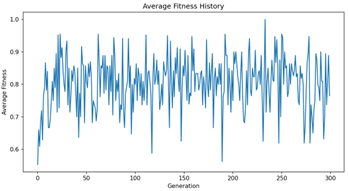
\includegraphics[width=\textwidth]{vt_only.png}
        % \caption{Subfigure 1}
        % \label{fig:sub1}
    \end{subfigure}
    % \hfill
    \begin{subfigure}[b]{0.05\textwidth}
        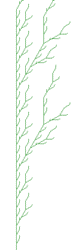
\includegraphics[width=\textwidth]{vt_only_dr.png}
        % \caption{Subfigure 2}
        % \label{fig:sub2}
    \end{subfigure}
    \vspace{0.5cm}
    \caption{$w_{vt}, w_{bs}, w_{s}, w_{pha}, w_{bp} = 100, 0, 0, 0, 0$}
    \label{fig:subfigures}
\end{figure}

\subsubsection{Bilateral Symmetry}
\begin{figure}[H]
    \centering
    \begin{subfigure}[b]{0.3\textwidth}
        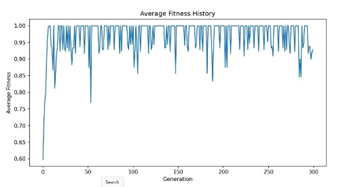
\includegraphics[width=\textwidth]{Sym_only_oa.png}
        % \caption{Subfigure 1}
        % \label{fig:sub1}
    \end{subfigure}
    % \hfill
    \begin{subfigure}[b]{0.1\textwidth}
        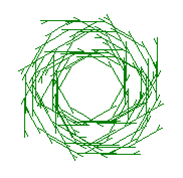
\includegraphics[width=\textwidth]{symm_only_dr.png}
        % \caption{Subfigure 2}
        % \label{fig:sub2}
    \end{subfigure}
    \begin{subfigure}[b]{0.1\textwidth}
        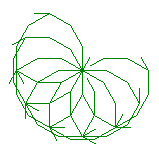
\includegraphics[width=\textwidth]{symm_only_dr2.png}
        % \caption{Subfigure 2}
        % \label{fig:sub2}
    \end{subfigure}
    \vspace{0.5cm}
    \caption{$w_{vt}, w_{bs}, w_{s}, w_{pha}, w_{bp} = 0, 100, 0, 0, 0$}
    \label{fig:subfigures}
\end{figure}

\subsubsection{Photon Gathering Ability}
\begin{figure}[H]
    \centering
    \begin{subfigure}[b]{0.3\textwidth}
        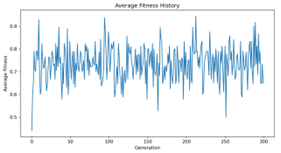
\includegraphics[width=\textwidth]{pg_only.png}
        % \caption{Subfigure 1}
        % \label{fig:sub1}
    \end{subfigure}
    % \hfill
    \begin{subfigure}[b]{0.1\textwidth}
        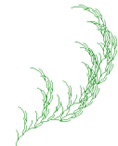
\includegraphics[width=\textwidth]{pg_only_dr.png}
        % \caption{Subfigure 2}
        % \label{fig:sub2}
    \end{subfigure}

    \vspace{0.5cm}
    \caption{$w_{vt}, w_{bs}, w_{s}, w_{pha}, w_{bp} = 0, 0, 0, 100, 0$}
    \label{fig:subfigures}
\end{figure}

\subsubsection{Stability}
\begin{figure}[H]
    \centering
    \begin{subfigure}[b]{0.3\textwidth}
        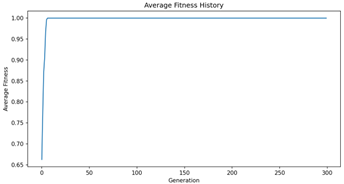
\includegraphics[width=\textwidth]{s_only.png}
        % \caption{Subfigure 1}
        % \label{fig:sub1}
    \end{subfigure}
    % \hfill
    \begin{subfigure}[b]{0.1\textwidth}
        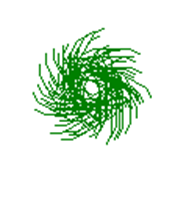
\includegraphics[width=\textwidth]{s_only_dr.png}
        % \caption{Subfigure 2}
        % \label{fig:sub2}
    \end{subfigure}

    \vspace{0.5cm}
    \caption{$w_{vt}, w_{bs}, w_{s}, w_{pha}, w_{bp} = 0, 0, 100, 0, 0$}
    \label{fig:subfigures}
\end{figure}

\subsubsection{Braching Proliferation}
\begin{figure}[H]
    \centering
    \begin{subfigure}[b]{0.3\textwidth}
        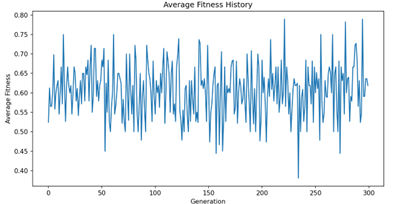
\includegraphics[width=\textwidth]{bp_only.png}
        % \caption{Subfigure 1}
        % \label{fig:sub1}
    \end{subfigure}
    % \hfill
    \begin{subfigure}[b]{0.1\textwidth}
        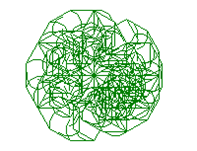
\includegraphics[width=\textwidth]{bp_only_dr.png}
        % \caption{Subfigure 2}
        % \label{fig:sub2}
    \end{subfigure}

    \vspace{0.5cm}
    \caption{$w_{vt}, w_{bs}, w_{s}, w_{pha}, w_{bp} = 0, 0, 100, 0, 0$}
    \label{fig:subfigures}
\end{figure}



\subsection{Block Mutation vs Symbol Mutation}

We implemented our system using both block mutation and symbol mutation. Figure~\ref{fig:mutation_comparison} and Figure~\ref{fig:mutation_comparison1}shows the comparison between the two mutation methods.

\begin{figure}[H]
    \centering
    \begin{subfigure}[b]{0.3\textwidth}
        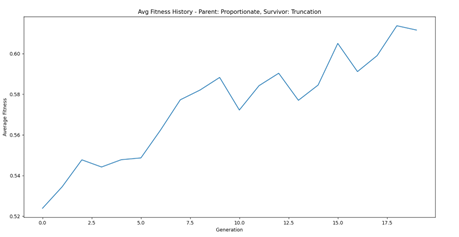
\includegraphics[width=\textwidth]{block1.png}
        % \caption{Subfigure 1}
        % \label{fig:sub1}
    \end{subfigure}
    % \hfill
    \begin{subfigure}[b]{0.1\textwidth}
        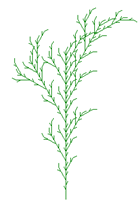
\includegraphics[width=\textwidth]{tree_block2.png}
        % \caption{Subfigure 2}
        % \label{fig:sub2}
    \end{subfigure}

    \vspace{0.5cm}
    \caption{$w_{vt}, w_{bs}, w_{s}, w_{pha}, w_{bp} = 100, 90, 40, 0, 80$}
    \label{fig:mutation_comparison}
\end{figure}

\begin{figure}[H]
    \centering
    \begin{subfigure}[b]{0.3\textwidth}
        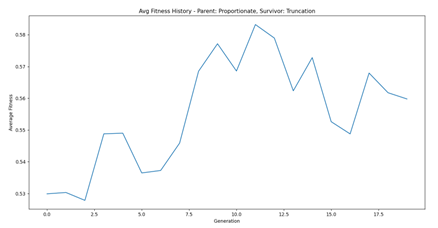
\includegraphics[width=\textwidth]{symbol.png}
        % \caption{Subfigure 1}
        % \label{fig:sub1}
    \end{subfigure}
    % \hfill
    \begin{subfigure}[b]{0.1\textwidth}
        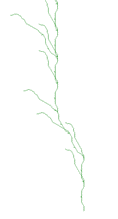
\includegraphics[width=\textwidth]{tree_sym.png}
        % \caption{Subfigure 2}
        % \label{fig:sub2}
    \end{subfigure}

    \vspace{0.5cm}
    \caption{$w_{vt}, w_{bs}, w_{s}, w_{pha}, w_{bp} = 100, 90, 40, 0, 80$}
    \label{fig:mutation_comparison1}
\end{figure}


We can observe from the figures that when we implemented the system with block mutation, it yielded better results compared to symbol mutation. This can be attributed to the fact that block mutation replaces a block of symbols rather than just a single symbol, allowing for larger-scale changes in the chromosome, which makes the population more diverse.


\subsection{Survivor Rank Based vs Survivor Truncation}

\begin{figure}[H]
    \centering
    \begin{subfigure}[b]{0.3\textwidth}
        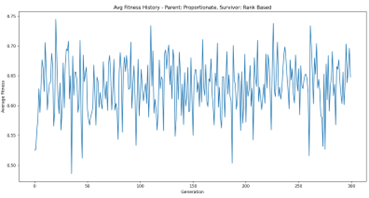
\includegraphics[width=\textwidth]{image2.png}
        % \caption{Subfigure 1}
        % \label{fig:sub1}
    \end{subfigure}
    % \hfill
    \begin{subfigure}[b]{0.1\textwidth}
        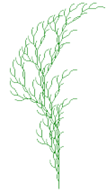
\includegraphics[width=\textwidth]{img2.png}
        % \caption{Subfigure 2}
        % \label{fig:sub2}
    \end{subfigure}

    \vspace{0.5cm}
    \caption{$w_{vt}, w_{bs}, w_{s}, w_{pha}, w_{bp} = 100, 90, 40, 0, 80$}
    \label{fig:mutation_comparison}
\end{figure}

\begin{figure}[H]
    \centering
    \begin{subfigure}[b]{0.3\textwidth}
        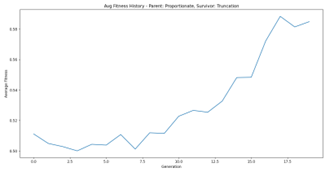
\includegraphics[width=\textwidth]{image1.png}
        % \caption{Subfigure 1}
        % \label{fig:sub1}
    \end{subfigure}
    % \hfill
    \begin{subfigure}[b]{0.1\textwidth}
        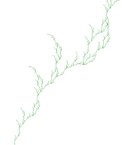
\includegraphics[width=\textwidth]{image.png}
        % \caption{Subfigure 2}
        % \label{fig:sub2}
    \end{subfigure}

    \vspace{0.5cm}
    \caption{$w_{vt}, w_{bs}, w_{s}, w_{pha}, w_{bp} = 100, 90, 40, 0, 80$}
    \label{fig:mutation_comparison}
\end{figure}

Implementing truncation in our system posed challenges, notably in the considerable time required for figure generation due to the significant increase in string length. Unlike truncation, this issue was not observed with the rank-based or any other survivor scheme. Due to limitations in computational resources, we could only implement truncation for 20 generations, compared to 300 generations in the case of rank-based selection. Despite this limitation, the figures clearly demonstrate that truncation outperforms rank-based selection by consistently selecting the fittest individuals, thus ensuring a higher overall performance.

\subsection{Parent Fitness Proportion vs Parent Tournament Selection}

\begin{figure}[H]
    \centering
    \begin{subfigure}[b]{0.3\textwidth}
        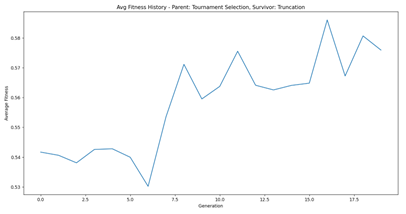
\includegraphics[width=\textwidth]{image3.png}
        % \caption{Subfigure 1}
        % \label{fig:sub1}
    \end{subfigure}
    % \hfill
    \begin{subfigure}[b]{0.1\textwidth}
        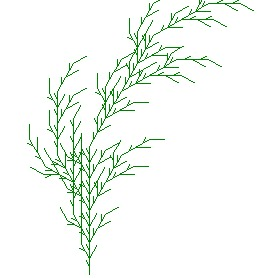
\includegraphics[width=\textwidth]{image6.png}
        % \caption{Subfigure 2}
        % \label{fig:sub2}
    \end{subfigure}

    \vspace{0.5cm}
    \caption{$w_{vt}, w_{bs}, w_{s}, w_{pha}, w_{bp} = 100, 90, 40, 0, 80$}
    \label{fig:mutation_comparison}
\end{figure}

\begin{figure}[H]
    \centering
    \begin{subfigure}[b]{0.3\textwidth}
        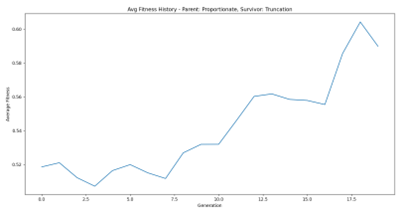
\includegraphics[width=\textwidth]{image5.png}
        % \caption{Subfigure 1}
        % \label{fig:sub1}
    \end{subfigure}
    % \hfill
    \begin{subfigure}[b]{0.1\textwidth}
        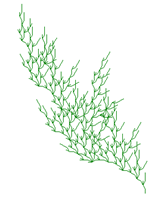
\includegraphics[width=\textwidth]{image7.png}
        % \caption{Subfigure 2}
        % \label{fig:sub2}
    \end{subfigure}

    \vspace{0.5cm}
    \caption{$w_{vt}, w_{bs}, w_{s}, w_{pha}, w_{bp} = 100, 90, 40, 0, 80$}
    \label{fig:mutation_comparison}
\end{figure}

In our system, we employed various parent selection schemes. However, when comparing tournament selection with fitness proportionate selection, the latter outperformed. This is because fitness proportionate selection consistently emphasizes choosing individuals based on their fitness, leading to a more directed evolutionary process. Conversely, tournament selection introduces randomness, potentially leading to suboptimal parent choices and slower convergence towards optimal solutions.




\section{Future Work}
In our implementation, a chromosome represents rule, which is dynamically updated by substitution in the genetic algorithm a certain number of itmes. This results in the updated string being increased by a significant factor in a very short amount of time. Thus, parent selection schemes that need to calculate the fitness of the entire, or a significant portion of the population take a considerable amount of time. In particular, the truncation scheme for parent selection shows significant performance degradation for very small number of generations of about 20 due to the increased string length. A similar degradation is seen in the fitness proportionate selection scheme, which also requires the fitness of the entire population to be calculated. Due to this, we were unable to run the truncation scheme for more than 20 generations, compared to 300 generations for other selection schemes. Access to more computational resources instead of our laptops, such as a high-performance computer or computing cluster would allow us to run the truncation scheme for a longer period of time, and potentially observe better results. 

Further, most of our testing for the new rules was done for the tree-based structure. The fitness functions were also designed to optimize the tree-based structure. The same is being used for the Sierpenski triangle and the Dragon Curve. Future work could include specifically testing the new rules for these structures, and designing new and better rules and fitness functions tailored to these structures based on the patterns that they exhibit. This would undoubtedly give even better results for these structures.

Lastly, the colour of the structure can also be taken into account when designing the fitness function. This can be used as a parameter in the fitness function to determine the fitness of the structure. Taking the colour as a parameter and evolving it would allow for the generation of more aesthetic, visually appealing, beautiful, and even realistic structures. This could also result in taking a step towards the generation of realistic flora.

% \input{Functioning.tex}
% \input{Experimental Results}


% \input{conclusion}

\bibliographystyle{ieeetr}
\bibliography{ref}

\end{document}

